\setcounter{framenumber}{372}
\begin{frame}
  \LectureNo{12}
	\maketitle
\end{frame}

\begin{frame}{Overview}
\tableofcontents
\end{frame}

\section{Course Summary}
\begin{frame}{Course Summary}
	
  \begin{itemize}

    \item We studied validity as truth-preservation:
      \begin{itemize}
      \item An inference is valid iff in every situation where the
        premises are true, the conclusion is true as well.
      \end{itemize}
      \item We developed this idea into a programmable, formal theory.
      \item We did this in three steps:
        \begin{itemize}
        \item In syntax, we abstracted from natural to formal
          languages.
        \item In semantics, we abstracted from possible situations to models.
          
            \item In proof-theory, we studied symbolic derivation systems.
            \end{itemize}
              \item We showed that our derivation systems are sound
                and complete:
                \begin{itemize}
                \item We can derive the conclusion from the premises
                  in all and only the valid inferences.
                \end{itemize}
                \item We did all this for two logical systems:
            \begin{itemize}
            \item classical propositional logic
              \item classical first-order logic
              \end{itemize}
                \item We proved that propositional logic is decidable
                  and observed that first-order logic is not.
										
	\end{itemize}

\end{frame}

\begin{frame}{Regrets?}

\begin{center}
  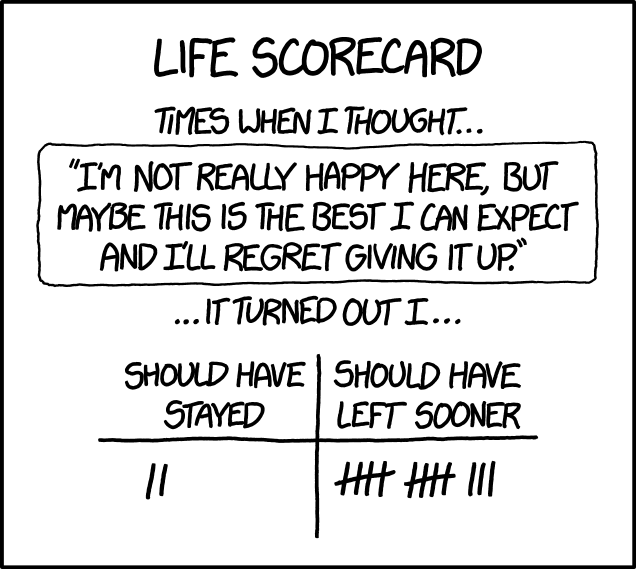
\includegraphics[width=30ex]{xkcd-regret}\\
  {\tiny \textcopyright~\url{https://www.xkcd.com/1768/}, CC BY-NC 2.5}
\end{center}

\end{frame}


\section{The Road Not Taken}
\subsection{More Theorems}

\begin{frame}{More Theorems} 

\begin{center}
  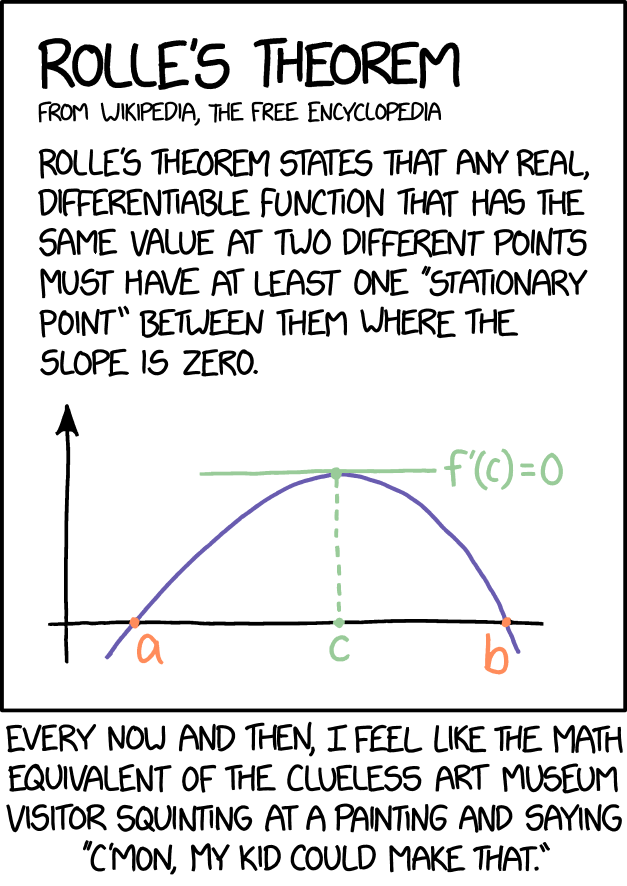
\includegraphics[width=30ex]{xkcd-rolle}\\
  {\tiny \textcopyright~\url{https://www.xkcd.com/2042/}, CC BY-NC 2.5}
\end{center}

\end{frame}

\subsubsection{Post Completeness}

\begin{frame}{Post Completeness}

  \begin{itemize}
  \item Remember that a logical law is a universal claim about
    $\vDash$, such as: \[\phi\land \psi\vDash
      \phi\lor \psi\]

  \item For each logic, we can consider the set of its laws, it's
    going to be a set of \emph{schemas} like the one above.

  \item For a logic $L$, let's denote the set of its laws by
    $LAWS_L$.

   \item We write $LAWS_{CPL}$ for the set of laws of classical
    propositional logic.

  \item \textbf{Theorem} (Post Completeness)\textbf{.} There exists no
    non-trivial propositional logic $L$ such that $LAWS_{CPL}\subset
    LAWS_L$. 
    
  \end{itemize}
  
\end{frame}

\subsubsection{Truth-Functional Completeness}
\begin{frame}{Truth-Functional Completeness}

  \begin{itemize}

  \item In propositional logic, why did we choose
    $\neg,\land,\lor,\to,\leftrightarrow$?

  \item Remember an $n$-ary truth-function is a function
    \[f:\{0,1\}^n\to \{0,1\}.\] 
    
  \item We say that a formula $\phi(p_1, \mathellipsis, p_n)$
    \emph{represents} $f:\{0,1\}^n\to \{0,1\}$ iff for all valuations
    $v$, \[\llbracket \phi\rrbracket_v=f(v(p_1),\mathellipsis,
      v(p_n))\]

  \item \emph{Examples}:
    \begin{itemize}
    \item $\neg p_1$ represents $f_\neg$
    \item $p_1\circ p_2$ represents $f_\circ$
    \item $\neg p_1\lor p_2$ represents $f_\to$!
    \item $\neg (\neg p_1\lor \neg p_2)$ represents $f_\land$!
    \end{itemize}

    \item \textbf{Theorem} (Truth-Functional Completeness)\textbf{.}
      For \emph{every} $n$-ary truth-function $f$, there exists a
      formula $\phi(p_1, \mathellipsis, p_n)$ that represents $f$. 

  \end{itemize}

\end{frame}

\begin{frame}{Complete Sets of Connectives}

  \begin{itemize}
  \item If $X$ is a set of connectives, we define $\mathcal{L}_X$ to
    be the language with only connectives in $X$.

    \item We say that $X$ is \emph{truth-functionally
        complete} iff for every $n$-ary truth-function $f$, there
        exists a formula $\phi(p_1, \mathellipsis,
        p_n)\in\mathcal{L}_X$ that represents $f$.

      \item \textbf{Proposition.} The following sets \emph{are}
        truth-functionally complete:
        \begin{enumerate}[1.]
        \item $\{\neg,\lor\}$
        \item $\{\neg,\land\}$
        \item $\{\neg, \to\}$
        \end{enumerate}
      \item \textbf{Observation.} The following sets are \emph{not}
        truth-functionally complete:
        \begin{enumerate}[1.]
        \item $\{\land,\lor\}$
        \item $\{\land,\to\}$
        \item $\{\lor, \to\}$
        \item $\{\land,\lor,\leftrightarrow\}$
        \item $\{\neg, \leftrightarrow\}$
        \end{enumerate}
        \item \textbf{Lemma.} If $X$ is truth-functionally
          complete and $X\subseteq Y$, then $Y$ is truth-functionally complete.
  \end{itemize}
  
\end{frame}

\begin{frame}{Some Weird Complete Connectives}

  \begin{itemize}

    \item Consider the language $\mathcal{L}_|$ which is defined over
      $\mathcal{P}$ with the BNF \[\phi::=p~|~(\phi~|~\phi).\]

      \item The connective $|$ is called the \emph{Sheffer stroke}. It expresses the
        following truth-function:
        truth-function:

        \begin{center}
          \begin{tabular}[h!]{c | c c}
            $f_|$ & 0 & 1\\\hline
            0     & 1 & 1\\
            1     & 1 & 0
          \end{tabular}
        \end{center}
       \item For the semantics, we say that \[\llbracket
         (\phi~|~\psi)\rrbracket_v=f_|(\llbracket \phi\rrbracket_v,
         \llbracket\psi\rrbracket_v)\]

       \item \textbf{Theorem.} The set $\{|\}$ is truth-functionally
         complete.

         \item If we want to build logic hardware, we only need to
           hardwire a truth-functionally complete set of connectives.
    
  \end{itemize}
  
\end{frame}

\subsubsection{Disjunctive and Conjunctive Normal Forms}
\begin{frame}{Disjunctive and Conjunctive Normal Forms}

  \begin{itemize}

  \item A \emph{literal} is a sentence letter or its negation:
    $p,\neg, q, \neg q, \mathellipsis$.

   \item A \emph{conjunctive form} is a formula of the
     form: \[l_1\land \mathellipsis\land l_n,\] where $l_1,
     \mathellipsis, l_n$ are literals.

    \item  A \emph{disjunctive form} is a formula of the
     form: \[l_1\lor \mathellipsis\lor l_n,\] where $l_1,
     \mathellipsis, l_n$ are literals.

     \item A formula $\phi$ is in \emph{disjunctive
         normal form} (DNF) iff $\phi$ is of the
       form \[\phi_1\lor\mathellipsis\lor\phi_n,\] where the $\phi_1,
       \mathellipsis, \phi_n$ are conjunctive forms.

       \item A formula $\phi$ is in \emph{conjunctive
         normal form} (CNF) iff $\phi$ is of the
       form \[\phi_1\land\mathellipsis\land\phi_n,\] where the $\phi_1,
       \mathellipsis, \phi_n$ are conjunctive forms.

    
  \end{itemize}

\end{frame}

\begin{frame}{The DNF Theorem and the CNF Theorem}

  \begin{itemize}
  \item \textbf{Theorem} (DNF/CNF Theorem)\textbf{.} For every formula
    $\phi\in\mathcal{L}$, there exists a formula $\psi$ in DNF (CNF)
    such that $\phi\equi \psi$.

   \item \emph{Proof}: A fantastic exercise for inductive proofs! $\square$

  \item \emph{Example}:  $(p\to \neg q)\land r$

    \begin{itemize}

    \item DNF: $(\neg p\land r)\lor (\neg q\land r)$

      \item CNF:$(\neg p\lor \neg q)\land r$

      \end{itemize}

     \item Normal forms are fantastic for reasoning, \emph{especially}
       automated reasoning (as we'll see later). 
    
  \end{itemize}

\end{frame}

\subsubsection{Prenex Normal Form}
\begin{frame}{Prenex Normal Form}

  \begin{itemize}
  \item Turning to first-order logic, we also have normal forms here.

  \item A formula $\phi$ is said to be in \emph{prenex normal form}
    (PNF) 
    iff $\phi$ is of the form \[Q_1x_1\mathellipsis Q_nx_n\phi',\]
    where $\phi'$ doesn't contain any quantifiers.

   \item \textbf{Theorem} (PNF Theorem)\textbf{.} For every formula
   $\phi\in\mathcal{L}$ there exists a formula $\psi$ in prenex normal
   form such that $\phi\equi \psi$.

 \item \emph{Example}: $\forall x(\exists yP(y)\lor (\exists zQ(z)\to
   R(x)))$

   \begin{itemize}
   \item PNF: $\forall x\exists y\forall z(P(y)\lor (Q(z)\to R(x)))$
   \end{itemize}

  \end{itemize}
  
\end{frame}


\subsubsection{L\"owenheim-Skolem Theorem}
\begin{frame}{L\"owenheim-Skolem Theorem}

  \begin{itemize}

  \item In mathematics, we say that two sets $X$ and $Y$ have the same
    \emph{cardinality} (i.e. size) iff there is a way of putting the
    members of $X$ and $Y$ in a one-to-one correspondence.

  \item \emph{Example}:

    \begin{center}
      \begin{tabular}[h!]{c c c c c}
        Natural Numbers:  &
                            0        &       1       &      2       & \dots\\
       &  $\updownarrow$  & $\updownarrow$  & $\updownarrow$ & \dots\\
       Odd Numbers:   &   1        &       3       &      5       & \dots
      \end{tabular}
    \end{center}

    There are as many even numbers as there are odd numbers.

    \item We say that the cardinality of $X$ is \emph{strictly
        smaller} than that of $Y$ iff there exists a $Z\subseteq Y$
      with the same cardinality as $X$ but no $Z\subseteq X$ with the
      same cardinality as $Y$.
      

    \item \textbf{Theorem} (Cantor)\textbf{.} The cardinality of
      $\mathbb{N}$ is strictly smaller than the cardinality of
      $\mathbb{R}$.

    \item \textbf{Theorem} (L\"owenheim and Skolem)\textbf{.} If a set
      of first-order formulas $\Gamma$ is satisfiable in a model
      $\mathcal{M}$, then there exists a model $\mathcal{M}'$ such
      that the cardinality of $D^\mathcal{M}$ is at most the
      cardinality of $\mathbb{N}$.
    
  \end{itemize}
  
\end{frame}

\subsubsection{G\"odel's Incompleteness Theorem}
\begin{frame}{G\"odel's Incompleteness Theorem}

  \begin{itemize}
  \item Peano Arithmetic is the standard theory of the natural numbers.
  \item The axioms of Peano Arithmetic, $PA$, are:
    \begin{itemize}
    \item $\neg \exists x~S(x)=0$
    \item $\forall x\forall y(S(x)=S(y)\to x=y)$
    \item $(\phi)[x:=0]\land \forall x(\phi\to (\phi)[x:=S(x)])\to
      \forall x\phi$ for all formulas $\phi$
     \item $\forall x(x+0=x)$
     \item $\forall x\forall y(x+S(y)=S(x+y))$
     \item $\forall x(x\cdot 0=0)$
     \item $\forall x\forall y(x\cdot S(y)=x+(x\cdot y)$
    \end{itemize}

   \item Remember the standard model $\mathcal{M}_{PA}$ for
     $\mathcal{S}_{PA}$:

     \begin{itemize}
     \item \textbf{Theorem.} If $PA\vdash \phi$, then
       $\mathcal{M}_{PA}\vDash\phi$.

      
     \end{itemize}

      \item \textbf{Theorem} (G\"odel's Second Incompleteness
         Theorem)\textbf{.} There exists a formula
       $\phi\in\mathcal{L}_{PA}$ such that $\mathcal{M}_{PA}\vDash A$
       but for no satisfiable $\Gamma\supseteq PA$, $\Gamma\vdash \phi$

  \end{itemize}

\end{frame}

\begin{frame}{Proof (Sketch)}

  \begin{itemize}
  \item We can define for each formula $\phi\in\mathcal{L}_{PA}$ a
    term $\ulcorner \phi\urcorner\in\mathcal{T}_{PA}$.
  \item If $PA\subseteq \Gamma$, then it is possible to find a formula
    $Prov_\Gamma\in\mathcal{L}_{PA}$ with $x$ free  such
    that \[PA\vdash (Prov_\Gamma)[x:=\ulcorner \phi\urcorner]\text{
        iff }\Gamma\vdash\phi\]
   \item For each $\Gamma\supseteq PA$ it is possible to find a formula
     $\lambda_\Gamma$ such that
     \[\Gamma\vdash \lambda_\Gamma
       \leftrightarrow (\neg
       Prov_\Gamma)[x:=\ulcorner \lambda_\Gamma\urcorner]\]

   \item $\lambda_\Gamma$ ``says of itself'' that its not provable.

   \item $\lambda_\Gamma$ can't be provable from consistent $\Gamma$:

     \begin{itemize}
     \item If $\Gamma\vdash \lambda_\Gamma$, then: \[\Gamma\vdash
       (Prov_\Gamma)[x:=\ulcorner\lambda_\Gamma\urcorner]\]\[\Gamma\vdash
       (\neg Prov_\Gamma)[x:=\ulcorner\lambda_\Gamma\urcorner]\] 
   \end{itemize}

 \item So $\Gamma\nvdash \lambda_\Gamma$.

   \item But that's what $\lambda_\Gamma$ ``says,'' so
     $\mathcal{M}_B\vDash \lambda_\Gamma$.
  \end{itemize}
  
\end{frame}

\subsubsection{Lindstr\"om's Theorem}
\begin{frame}{Lindst\"om's Theorem}

  \begin{itemize}

  \item \textbf{Theorem} (Compactness)\textbf{.} For each $\Gamma$, if
    $\Gamma\vdash\phi$, then there exists a finite
    $\Gamma'\subseteq\Gamma$ such that $\Gamma'\vdash\phi$.

  \item \emph{Proof}. As in propositional logic, via tableaux.

   \item \textbf{Theorem} (Lindstr\"om's Theorem). There is no
     non-trivial logic $L$ for which the L\"owenheim-Skolem theorem
     and the Compactness theorem holds and $LAWS_{CFOL}\subset
     LAWS_L$ (where $CFOL$ is classical first-order logic).
    
  \end{itemize}
  
\end{frame}

\begin{frame}{Applications of Compactness}

  \begin{itemize}
  \item A simple corollary from compactness is the \emph{semantic}
    compactness theorem:
    \begin{itemize}
    \item For all $\Gamma$, if each finite subset
      $\Gamma'\subseteq\Gamma$ is satisfiable, then $\Gamma$ is satisfiable.
    \end{itemize}

    \item This can be used to construct a model for $PA$ with
      $\infty$:

      \begin{itemize}
      \item We know that $PA$ is satisfiable.
      \item Consider $PA\cup\{n\neq \infty:n\in\mathcal{T}_{PA}\}$
      \item Clearly each finite subset of this set is satisfiable.
      \item So the whole set is satisfiable.
        
      \end{itemize}
  \end{itemize}
  
\end{frame}

\subsection{Resolution}
\begin{frame}{Resolution}

  \begin{itemize}
  \item Given that you now understand tableaux, you can easily learn
    \emph{resolution}.

  \item We want to formulate a decision procedure for CPL:

    \begin{itemize}
    \item  In order to to check $\phi$ for validity, we first find the
      CNF of $\neg\phi$: \[\phi_1\land \mathellipsis\land\phi_n\]
    \item Consider the set $\{\phi_1, \mathellipsis,\phi_n\}$.
    \item We now repeatedly apply the following rule to its members:
      
      \begin{center}
        \begin{tabular}{c}
        \infer{\phi_1\lor \mathellipsis\lor\phi_n\lor\psi_1\lor\mathellipsis\lor\psi_n}{\phi_1\lor \mathellipsis\lor
          \phi\lor\mathellipsis\lor\phi_n & \psi_1\lor \mathellipsis\lor
                                            \neg\phi\lor\mathellipsis\lor\psi_m}
        \end{tabular}
      \end{center}
      \item Whenever we come across a formula \[\phi_1\lor
        \mathellipsis
        \lor\phi\lor\mathellipsis\lor\neg\phi\lor\mathellipsis\lor\phi_n\]
      we eliminate it.
     \item If we can derive the empty expression $nil$, then $\phi$ is
       valid; if we can't derive $nil$ (after all possible
       applications of the resolution rule), then $\phi$ is invalid.
    \end{itemize}

      
  \end{itemize}
  
\end{frame}
             

\section{Logic in AI}

\begin{frame}{Logic in AI}


    \begin{quote}
     Logical AI involves representing knowledge of an agent’s world,
     its goals and the current situation by sentences in logic. The
     agent decides what to do by inferring that a certain action or
     course of action is appropriate to achieve the goals.
     \begin{flushright}
       (McCarthy 2000)
     \end{flushright}
    \end{quote}
    
\end{frame}


\begin{frame}{Logic as Machine Learning}

  \begin{itemize}
  \item We know that this doesn't work very well.

    \item Agents that use logic to reason about perception, to learn
      things about the world, to reach goals, etc. are ``clunky.''

      \begin{itemize}

      \item Plato: $\forall x(x$ is human iff $\neg(x\text{ has feathers}\land
     x\text{ has two legs}))$

      \item Diogenes: [plucks chicken]

      \end{itemize}

      \item So why do we study logic in the first place?
  \end{itemize}
  
\end{frame}

\begin{frame}{Logic as Foundations}%$

  \begin{itemize}
  \item Linguistics:
  \begin{itemize}
  \item Logical syntax is the foundation of formal grammar ($\leadsto$
    Chomsky grammars)
  \item Logical semantics is the foundation for formal semantics
    ($\leadsto$ Montague semantics)
  \end{itemize}
  \item Psychology:
    \begin{itemize}
    \item Models of reasoning need to take valid reasoning into
      account.
    \end{itemize}
    \item Computer science:
      \begin{itemize}
      \item Programming languages are (imperative) formal languages.
       \item Understanding them involves semantics.
         \item Evaluating expressions is essentially 
         \item There is a precise correspondence between proofs and
           programs ($\leadsto$ Curry-Howard correspondence) 
      \end{itemize}
  \end{itemize}
  
\end{frame}

\begin{frame}{Logic as Conditions}

  \begin{itemize}
  \item One of the main uses of (first-order) logic is to express
    conditions on models:

    \begin{itemize}
    \item $\mathcal{M}\vDash \forall xR(x,x)$ iff $(R^\mathcal{M}$ 

      \item More generally, we want to find formulas $\phi$ such that
        a model $\mathcal{M}$ has a property iff $\mathcal{M}\vDash\phi$.
    \end{itemize}

    \item This is essentially the reason why mathematics is formulated
      in first-order logic:
      \begin{itemize}
      \item We express properties of mathematical objects using
        first-order formulas.
      \end{itemize}
      
      \item AI is (on one way of looking at it) a modeling project:
        \begin{itemize}
        \item We're building models of intelligent systems.
        \end{itemize}
       \item These models need to satisfy certain constraints:
         \begin{itemize}
           \item Practicality constraints
           \item Real world constraints
             \item Normative constraints
         \end{itemize}
         \item These constraints are formulated in \dots logic!

  \end{itemize}
  
\end{frame}

\begin{frame}{Outlook}

What comes next?
  
  \begin{itemize}
  \item You'll all take \texttt{Modale Logica voor KI (KI3V19001)}, in
    which you'll extend logical treatments to relational systems:
    \begin{itemize}
    \item $\square \phi$ means that $\phi$ is true at all stages
      \item $\lozenge\phi$ means that $\phi$ is true at some stages
      \end{itemize}
      \item Some of you will choose the track \texttt{Reasoning and
          Language}:
        \begin{itemize}
        \item \texttt{Logische Complexiteit (KI3V12013)}
          \item \texttt{Semantics(KI3V12014)}
          \end{itemize}
          \item You'll study more mathematics and set theory in
            \texttt{Wiskunde voor KI (KI1V13005)}
  \end{itemize}
  
\end{frame}


\begin{frame}
  
\begin{center}
  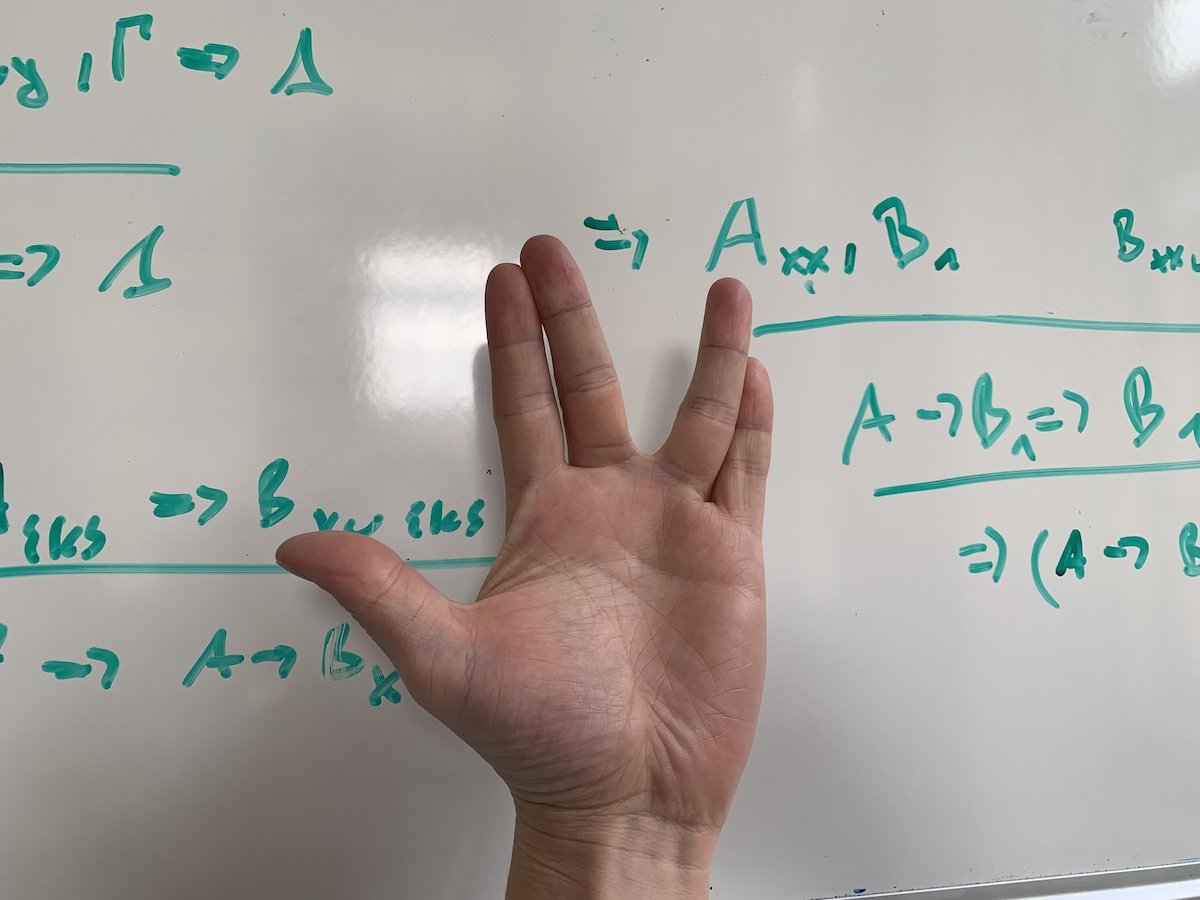
\includegraphics[width=40ex]{llap}
\end{center}

\end{frame}
